\chapter{SpTRSV算法的设计与实现}

\section{实现并行的SpTRSV的算法}

\subsection{一些准备操作}
该模块包含稀疏矩阵的读入。以及从矩阵中获得下三角矩阵。假设稀疏下三角矩阵求解的向量x\_ref,每个元素的值都为1.0。然后使用矩阵向量乘法,得到等式$Lx=b$右边的结果向量b。在SpTRSV算法并行求解之后,得到待求解的向量x,通过x与x\_ref对比,来验证结果的正确性。

\subsection{实现多核架构下的并行SpTRSV算法}

本算法基于CSC压缩格式的矩阵,将一列矩阵的计算抽象为一个任务。在预处理阶段同样只需统计每个任务的前置依赖,见伪代码\ref{SpTRSV-Preprocess}。该算法使用了一个并行的循环,拥有很好的扩展性,占总体运行的时间可以忽略不记。

\begin{algorithm}[htbp]
    \caption{并行SpTRSV算法预处理阶段伪代码\label{SpTRSV-Preprocess}}
    \SetKw{atomic-add}{atomic-add} 
    \SetKw{atomic-sub}{atomic-sub} 
    \SetKw{Parallel}{Parallel} 
    \SetKwProg{Fn}{Function}{ is}{end}
    malloc(*left\_sum, *in\_degree, n)\;
    memset(*left\_sum, *in\_degree, 0)\;
    \Fn{Preprocess()}{
        \Parallel \For{i = 0; i < nnz; i++}{ 
            atomic-add(\&in\_degree[row\_idx[i]], 1) \; 
        }
    }
\end{algorithm}

在计算阶段,多个线程从索引0开始依次分配,进行并行计算。首先通过一个自旋等待来判断前置条件是否满足,该自旋等待使用CPU松弛的技术进行优化,通过一定量的空转,减少了处理器为了维护内存序带来的性能损失。当前置条件满足时,首先会进行向量x[i]的计算。接着需要计算后继任务j所对应的left\_sum[j]和in[j],后者用来表示后继任务有多少前置条件已经被满足。对于第二个循环,由于稀疏矩阵非零元分布特点的不同,在第二个循环可能出现负载不均衡的现象。通过打印第二个循环的任务个数,对于部分矩阵存在着严重的负载不均衡的现象,例如名为webbase的矩阵(该矩阵来自于佛罗里达大学的矩阵集合\cite{davis2011university}),该矩阵93\%的任务在第二个循环当中只需计算0次,1.3\%的任务在第二个循环中需要计算1次,剩下任务的计算次数从2次到28684次分布,存在着严重的负载不均衡的现象。sync-free的算法使用一个warp来处理一个任务,而一个wrap有32个线程,对于哪些计算数量为0的任务,这会导致计算资源的大量浪费。因此在任务进入计算阶段之前,先进行负载均衡的操作,详见\ref{section:fuzaijunheng}。

\begin{algorithm}[htbp]
    \caption{并行SpTRSV算法计算阶段伪代码\label{SpTRSV-Solve}}
    \SetKw{atomic-add}{atomic-add} 
    \SetKw{atomic-sub}{atomic-sub} 
    \SetKw{Parallel}{Parallel} 
    \SetKwProg{Fn}{Function}{ is}{end}
    \Fn{Solve()}{
        \Parallel \For(using one warp for one entry){int i = 0; i < n; i++}{
            int in\_degree\_this\_task = in\_degree[i] - 1 \;
            prefetch(\small{\&$val[col\_ptr[i]]$}) \;
            prefetch(\small{\&$b[i]$}) \;
            \While{in[i]\small$\neq$ in\_degree[i]}{
                Pause() \; \tcc{cpu relax}
            }

            \small{$x[i] \leftarrow (b[i]-left\_sum[i])/val[col ptr[i]]$}\;
            \For(one thread for one nonzero){j in \small{$[col\_ptr[i]+1], col\_ptr[i+1]-1$}}{
                atomic-add(\&left\_sum[rid], \small{$val[j] \times x[i]$}) \;
                atomic-add(\&in[rid], 1) \;
            }
        }
    }
\end{algorithm}

在算法\ref{SpTRSV-Solve}的第4行,使用了prefetch的预取指令。在循环等待之前将稀疏矩阵非零元的值以及方程组等式右边的向量b[]提前缓存到cache中。

\section{消除伪共享}

由于对数组left\_sum以及数组in[rid]会出现大量的并发访存,会出现伪共享的情况,应该通过padding的方式消除。这里选择使用gcc的编译属性\_\_attribute\_\_进行padding。

\begin{lstlisting}[caption={消除伪共享}]
struct Node{
    std::atomic<size_t> csrRowHisto_atomic {0};
    std::size_t idx = {0};
    VALUE_TYPE left_sum {0.0};
    VALUE_TYPE xi {0.0};
}__attribute__((aligned(128)));
\end{lstlisting}

\section{负载均衡}\label{section:fuzaijunheng}

J.Park\cite{park2014sparsifying}通过合并超级任务的方式来进行负载均衡。他将同一个level中的任务进行合并,使得每个线程所分得的超级任务有相似的计算量。这种做法适合在已经构建了任务依赖图之后的情况;并且在有些level会出现,任务数量小于线程数量,没法进行合并。出于这两点考虑,本文选择通过分割大任务的方式来进行负载均衡。设定一个上限upper\_size,将超过上限的任务进行分割。创建多个线程,每个线程平均处理m个任务,如图\ref{负载均衡示意图}。

\begin{figure}[htbp]
    \centering
    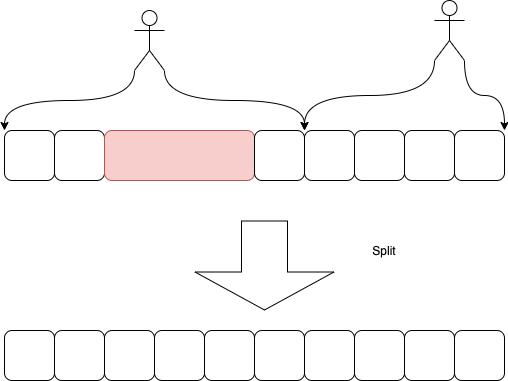
\includegraphics[width=0.7\textwidth]{loadbalance.png}
    \caption{负载均衡示意图}
    \label{负载均衡示意图}
\end{figure}

在后续测试中发现,随着矩阵规模的扩大,负载均衡算法会遇到内存带宽的瓶颈,导致由负载均衡的消耗远大于使用负载均衡带来的性能优化。对于这个问题本文提出了两种解决方案:一是利用NUMA架构的特性,提升内存带宽;而是在预处理阶段统计每个任务的计算任务负载情况的最大值和最小值。只对两者差距不是很大就不进行负载均衡。


\section{使用SIMD指令}

并行SpTRSV算法的第二个循环可以通过SIMD指令进行优化。由于ARM Neon只提供了128bit的向量寄存器,只能放下两个double和四个float,这里只对float类型的数据进行向量化计算的操作。算法流程为:首先用数据类型float32x\_t创建两个Neon寄存器变量vec\_xi、vec\_csaVal,该数据类型表示一个向量中有4个float32数据,分别表示由行号为i的未知数x组成的向量和稀疏矩阵一列上非零元组成的向量。将原来步长为1的循环,现在要修改为步长为4的循环。然后使用vld1q\_f32指令将稀疏矩阵中的4个非零元load进入vec\_csaVal寄存器当中,使用vld1q\_dup\_f32,将xi复制4份,load进vec\_xi寄存器中。之后使用vmulq\_f32,执行向量乘法的操作。最后使用vgetq\_lane\_f32(vec\_result),将向量乘法的结果从寄存器中取出,并写会内存当中。

在将结果写会内存的时候,由于一列上的非零元的行号都是离散的,因此对应产生结果的行号也不是连续的,这就导致本文们无法通过一个store命令直接将结果写如left\_sum中,而是需要分开进行独立的写操作。

\begin{lstlisting}[caption={SIMD指令优化}]
    float32x4_t vec_xi;
    float32x4_t vec_csaVal;
    vec_xi = vld1q_dup_f32(&xi);
    for each nonzero in column (step_size = 4) {
        result[0] = vgetq_lane_f32(vec_csaVal, 0);
        result[1] = vgetq_lane_f32(vec_csaVal, 1);
        result[2] = vgetq_lane_f32(vec_csaVal, 2);
        result[3] = vgetq_lane_f32(vec_csaVal, 3);
        STORE result;
    }
\end{lstlisting}

\section{使用LSE指令}

由于算法使用了大量的原子操作,例如对于left\_sum和in\_degree使用了很多的原子操作,使用原有争抢式的原子指令会对程序的性能产生消极影响。在开启LSE原子指令之前CAS操作需要通过LDXR和STXR并通过不断判断的方式实现,而在开启LSE只需一条casal指令,同样原子加法操作也只需一条LDADD指令。

具体实现方式为,通过编译器参数'-march=armv8-a+lse'来实现

\section{使用NUMA架构}

NUMA架构的优点是扩展了系统的内存带宽,提升了系统的CPU核心数目,缓解了缓存一致性的冲突。但是却带来了远程内存访问,延迟过高等缺陷。软件设计人员需要充分考虑并利用这个特性,否则会带来性能的损失。

通过numactl --hardware命令可以获得本机的numa硬件情况,本机使用的NUMA特性如图所示\ref{numaHardware}。从该图node distances可以看出远程访问的延迟可以为本地访问延迟的1.6至3.3倍。

\begin{figure}[htbp]
    \centering
    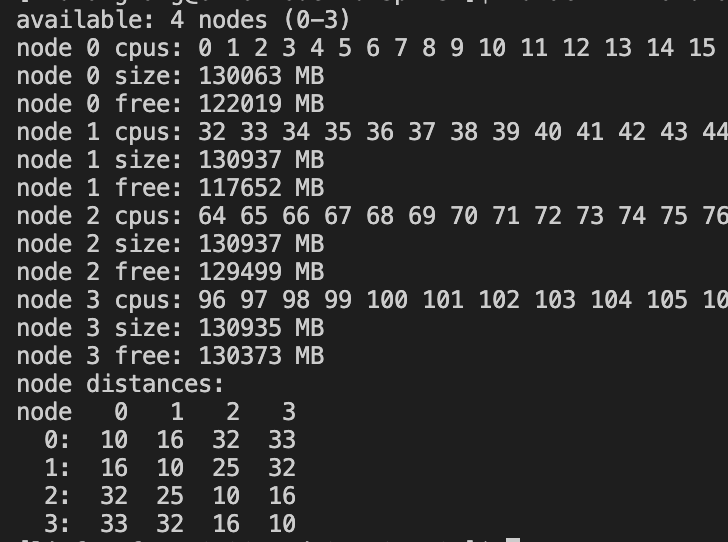
\includegraphics[width=0.7\textwidth]{numaHardware.png}
    \caption{本机所使用的硬件特性}
    \label{numaHardware}
\end{figure}

本算法使用的数据按照读写特征主要分为以下二类:
\begin{enumerate} \setlength{\itemsep}{0pt}
    \item 只读数据类型:稀疏的三个数组,cscCowPtr[]、cscRolIdx[]、cscVal[]以及等式$Lx=b$右边的向量b[]。
    \item 频繁通过原子操作读写:left\_sum[]、in\_degree[]、未知数向量x[]
\end{enumerate}

对于只读的数据类型本文主要通过创建数据副本的形式,将只读数据分成四分,分配到四个NUMA节点上。主要是通过通过Linux操作系统提供的C语言编程接口\cite{libnuma}libnuma中的void *numa\_alloc\_onnode(size\_t size, int node),接口参数int node表示指定结点的编号。线程首先通过sched\_getcpu()和numa\_node\_of\_cpu(cpuid),得到自己所在结点的信息,根据这个信息来访问局部数据。然而对于频繁通过原子操作读写的数据,由于数据读写的随机性,没法使用numa架构进行很好的优化。

总的来说,本文主要尝试了四种种NUMA策略。
\begin{enumerate} \setlength{\itemsep}{0pt}
    \item 使用numactl --cpunodebind,将所有任务都固定在一个结点上。
    \item 使用numactl --cpunodebind,将任务固定在两个距离相近的NUMA节点上。
    \item 使用numactl --interleave,将数据均匀分布在四个numa节点上。
    \item 创建只读数据副本,并将其分配到个结点上。
\end{enumerate}

经过测试发现对于小规模或者并行性第的稀疏矩阵固定在单一结点上性能是最好的。而对于规模较大并行性较好的稀疏矩阵,我采用策略4,也就是创建只读数据副本,并将数据与任务分配到多个节点上能获得约15\%的性能提升,详见\ref{NUMA架构对性能的影响}

\section{本章总结}

本章介绍了本算法的设计以及优化思路。包括一些程序读入,数据整理以及结果验证的辅助操作,基本的并行架构及其在此基础上的优化技巧。主要的优化技巧有:通过prefetch指令进行预缓存;使用CPU松弛技术提升自旋等待的整体性能;使用padding的方法消除伪共享;在分析矩阵任务负载不均衡的基础上提出了负载均衡的策略;使用SIMD指令进行优化;通过编译指令的方式开启LSE指令集,优化了原子操作的性能;以及针对NUMA架构进行了一系列的策略尝试优化。


\endinput